\documentclass[PICOReport.tex]{subfiles}

\begin{document}

%To cover: Galaxy Formation, Clusters, Reionization, point sources (probably moves to a new section called 'Legacy Science')

{\bf The Formation of the First Luminous Sources}\\
The reionization of the Universe, which according to current measurements takes place near a cosmic age of $\sim$700 million 
years~\citep{planckreion}, imprints multiple signals in the temperature and polarization of the CMB.  In polarization, the most 
important signal is an enhancement of power in the E-mode spectrum at large angular scales $\ell \simlt 20$. 
%scale $E$-mode power sourced by the scattering of the temperature quadrupole during this epoch.  
This signal gives a direct measurement of the optical depth to the reionization epoch $\tau$, and thus to the 
mean redshift of reionization $Z_{re}$, with very little degeneracy with other cosmological parameters; see Figure~\ref{fig:ReionizationPICO}. 
%In contrast, inference of $\tau$ from the $TT$ power spectrum is hindered by its direct degeneracy with the scalar fluctuation amplitude.  
The mean redshift of reionization $Z_{re}$ (when $50$\% of the cosmic volume was reionized) depends sensitively 
on the nature of the ionizing sources.  For example, it is currently unknown whether star-forming galaxies or more exotic 
sources such as supermassive black holes drove the reionization process.  \comor{is this THE question, or are there other 
examples? Would the answer change $Z_{re}$?}
%The PICO constraint on $\tau$ is converted to a constraint on $z_{re}$ in Fig.~\ref{fig:ReionizationPICO}, which is further discussed below.
Furthermore, the detailed shape of the low-$\ell$ $E$-mode power spectrum is sensitive to the reionization history 
itself (i.e., $d\tau/dz$), and will provide information beyond that captured in $\tau$ alone.  For example, it has been 
argued that \planck data show evidence for an extended tail of reionization out to $z \approx 15$-$20$~\cite{Miranda2017}.  
A cosmic-variance-limited measurement of the large-scale $E$ modes, as obtained by PICO, will settle this question.  
%The measurement of $\tau$ constrains the mean redshift of reionization, $z_{re}$ (i.e., when $50$\% of the cosmic volume was reionized), which depends sensitively on the nature of the ionizing sources.  For example, it is currently unknown whether star-forming galaxies or more exotic sources (e.g., supermassive black holes) drove the reionization process.  The PICO constraint on $\tau$ is converted to a constraint on $z_{re}$ in Fig.~\ref{fig:ReionizationPICO}, which is further discussed below.  %\comor{not sure about the comment in the parenthesis. $\tau$ is in the STM to 'distinguish between models that describe the formation of the earliest stars' , but that aspect is not highlighted here ...(??). the paragraph also doesn't reference Figure 3, should it?} 
 
Large-scale $EE$ power spectrum measurements are a unique and crucial observable for many aspects of cosmology \comor{which many}.  
If measurements of $\tau$ are not improved beyond the current uncertainties from {\em Planck}, inference of several new signals 
of cosmological physics (e.g., neutrino mass) will be severely hindered \comor{which other new signals}.  
PICO is the ideal experiment to make this measurement.  
Its noise level and frequency coverage permit a cosmic-variance-limited constraint on $\tau$, i.e., $\sigma(\tau) \approx 0.002$, which we have verified with explicit forecasts including foregrounds. 
% We verify this expectation via an explicit forecast following the methodology described in~\citet{errard_feeney_2015}, assuming PICO measurements of the $TT$, $TE$, $EE$, $BB$, and $\phi\phi$ power spectra, with the latter inferred via the iterative $EB$ estimator.  The polarized dust and synchrotron levels match those measured by {\em Planck}~\citep{PlanckFG2015}, including spatial variations, and are cleaned using a parametric maximum-likelihood approach.  Fitting a $\Lambda$CDM$+r$ model, for both the PICO ``requirements'' and ``CBE'' configurations, we find $\sigma(\tau) = 0.002$.  With the exquisite control of systematics needed for the much smaller primordial $BB$ signal, these are not a concern for $EE$ (and hence $\tau$).

In temperature, the most important imprint of reionization is that sourced at small angular scales by the ``patchy'' kinematic 
Sunyaev-Zel'dovich (kSZ) effect, due to the peculiar velocities of free electron bubbles around ionizing sources (e.g., galaxies or quasars).  
The total kSZ power spectrum receives contributions from both the patchy reionization signal and ``late-time'' sources, e.g., the intergalactic and 
intracluster media.  The reionization and late-time signals are expected to have comparable 
amplitudes~\citep{Shaw2012,MMS2012,Battaglia2013}.  With constraints on the late-time contribution from other 
information (e.g., cross-correlations), effective small-scale foreground removal, and with the primary CMB $TT$ power 
spectrum constrained by inference from the $EE$ power spectrum, it is possible to extract reionization constraints from the 
small-scale kSZ power spectrum~\citep{calabrese/etal/2014}.  The most directly constrained quantity is the duration of 
reionization, $\Delta z_{re}$. \comor{if pico is not providing kSZ constraints, only S3 does, there 
is no need to dwell on it at all, I think.  Nick, can you condense this?}

Fig.~\ref{fig:ReionizationPICO} presents forecasts for reionization constraints in the $z_{re}$-$\Delta z_{re}$ parameter space obtained 
from PICO's measurement of $\tau$ in combination with ground-based Stage-III (CMB-S3) constraints on the kSZ power spectrum.  
Constraints from existing Planck data and observations at other wavelengths are also presented.  The PICO measurement of $\tau$ 
is essential for breaking degeneracies \comor{does not appear to be borne out by the figure} and allowing simultaneous, 
precise constraints to be placed on both the mean redshift and 
duration of reionization.  Fig.~\ref{fig:ReionizationPICO} also shows curves of constant source efficiency (i.e., the efficiency of 
ionizing photon production) and constant intergalactic medium opacity (i.e., the photon mean free path).  PICO will allow 
simultaneous constraints to be placed on these physical parameters, yielding important information on the nature of the 
first luminous sources (e.g., star-forming galaxies or quasars predict significantly different values for these parameters).

\begin{figure}
\hspace{-0.in}
\parbox{3.1in}{\centerline {
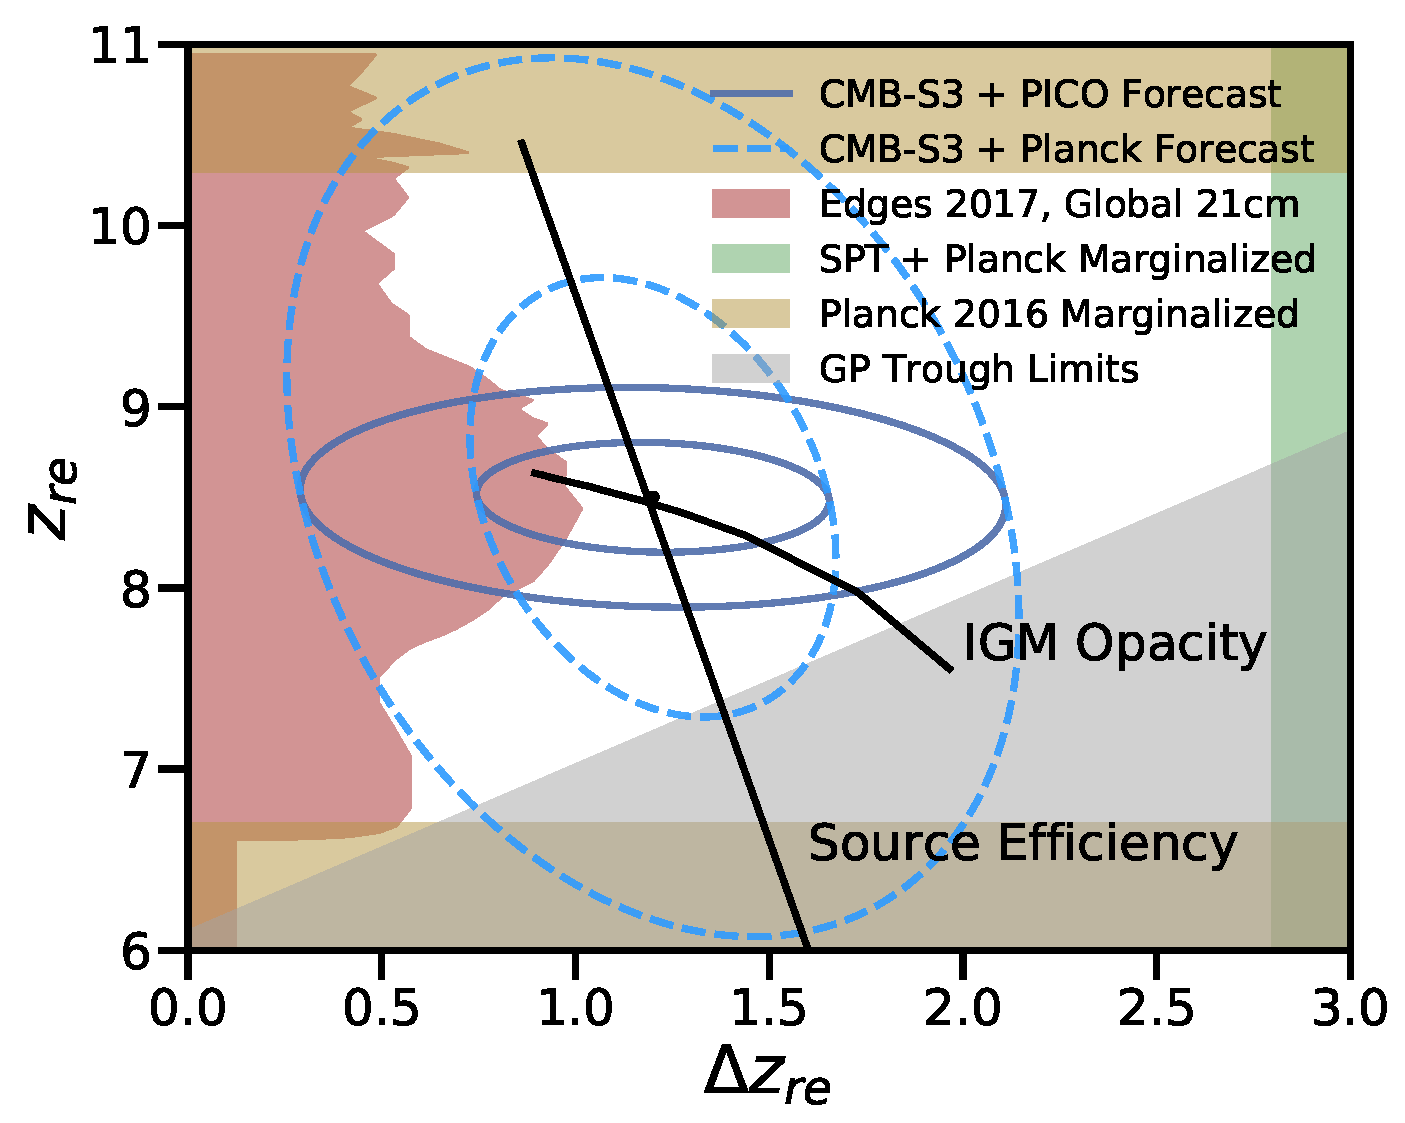
\includegraphics[width=3.0in]{images/Reionization_Contours_zbar_delz_PICO_NEW.pdf} } }
\hspace{0.in}
\parbox{3.5in}{
\caption{\label{fig:ReionizationPICO} Summary of constraints on the mean redshift and duration of reionization. The forecasts show 68\% and 95\% confidence-level contours for PICO combined with CMB-S3 experiments and Planck combined with CMB-S3 experiments (dark blue and dashed blue, respectively). The solid black lines illustrate how the IGM opacity and source efficiency model parameters map onto this parameter space. The forecasted PICO constraints are compared to: current exclusion limits for the mean redshift of reionization from Planck, shown by the yellow bands \citealp{planck2018:parameters}; recent exclusion limits from the global 21 cm signal measured by EDGES, shown with the red band \citealp{edges2017}; exclusion limits from measurements of the Gunn-Peterson trough from fully absorbed Lyman$\alpha$ in quasar spectra, shown by the grey band \citealp{Fan2006}; exclusion limit on the duration of reionization from Planck and SPT data, shown by the green band \citealp{planck_reio:2016}.} }
\vspace{-0.1in}
\end{figure}

In addition to these signals, reionization also leaves specific non-Gaussian signatures in the CMB.  In particular, patchy reionization 
induces non-trivial 4-point functions in both temperature~\citep{SmithFerraro2017} and polarization~\citep{DvorkinSmith2008}.  The 
temperature 4-point function can be used to separate reionization and late-time kSZ contributions.  Combinations of temperature and 
polarization data can be used to build quadratic estimators for reconstruction of the patchy $\tau$ field, analogous to CMB lensing 
reconstruction.  These estimators generally require high angular resolution, but also rely on foreground-cleaned CMB maps.  Thus, 
while PICO alone may not enable high S/N reconstructions, its high-frequency channels --- which have better than 2 arcmin 
resolution and observe at frequencies that have yet to be demonstrated from the ground --- will enable these estimators to be 
robustly applied to ground-based CMB data sets, a strong example of ground-space complementarity.
\comor{if pico is complementarity by {\it only} providing foreground maps at sufficiently high resolution, I think we should move 
this to the 'complementarity'. It is not a direct science goal or outcome.}

% JCH: I checked the Smith-Ferraro 4-pt estimator, and PICO does not have sufficient resolution to do this (see Fig. 3 of https://arxiv.org/pdf/1803.07036.pdf )

\comor{The Sections below need to be rearranged to match other Science Objective(s) from the STM, but to also relay the breadth of science reachable by PICO, even if those goals are not in the STM.}

{\bf Structure Formation via Gravitational Lensing}

Matter between us and the CMB last-scattering surface deflects the path of photons through gravitational lensing, encoding the 3-dimensional 
matter distribution across the entire visible universe onto a 2-dimensional image. The specific quantity being mapped is the projected gravitational 
potential $\phi$ that is lensing the CMB, commonly called the `lensing map', from which we form an angular power spectrum $C_{\ell}^{\phi \phi}$.  
Both the temperature and polarization maps of the CMB are affected by lensing, and subsequently the angular power spectra. One of the most 
pronounced effects is the existence of the `B-mode lensing power spectrum'; see Figure~\ref{??}.^\footnote{It is a result of graviational lensing of E-modes into B-modes.}  
While \planck  had a signal-to-noise ratio (SNR) of 40~\cite{ } \comor{map or phi-phi?}, 
the PICO combination of resolution, sensitivity and sky coverage \comor{is sky coverage important} enables a measurement with SNR of 638 and 737 
for the required and CBE configurations, respectively. When accounting for possible foreground contamination, its broad frequency coverage leads 
to a reduction of SNR of less than 20\%; see Figure~\ref{fig:lensingNoisePICO}.  
% say something about "the best measurement"...?
The value of such a deep lensing map is immense, as has already been seen with {\it Planck}. The lensing map is most sensitive to 
structures at redshift $z \simeq 2$ and down to scales of approximately ten arcminutes \comor{talk to Alex; there is a
comment about `wide range of angular scales'}.  
Tomographic cross-correlations of the lensing map with samples of galaxies and quasars will yield constraints 
on structure formation out to redshifts inaccessible to galaxy surveys or galaxy weak lensing maps on their own.
%, particularly through the high-S/N cross-correlation science that will be enabled.  
 These measurements will yield constraints on dark energy, modified gravity, and neutrino mass. Note that this neutrino mass constraint is 
 complementary to that inferred from the CMB lensing auto-power spectrum described earlier \comor{check how we referred to it
 earlier. do we have quantitative values for the constraints?}.  The measurements will constrain the properties of quasars and 
 other high-redshift astrophysics, e.g., a precise determination of the quasar bias (and hence host halo mass) as a function of their 
 properties, such as (non-)obscuration \comor{need to talk to Alex/Marcel about this}.  We provide further quantitative cross-correlation forecasts below.  

% Fig.~\ref{fig:lensingNoisePICO} shows per-mode noise curves for the reconstruction of CMB lensing from PICO, demonstrating the wide range of angular scales over which the matter density field will be  mapped.  \textbf{Add brief discussion of foreground robustness demonstrated in Fig.~\ref{fig:lensingNoisePICO}}

\begin{figure}
\hspace{-0.in}
\parbox{3.1in}{\centerline {
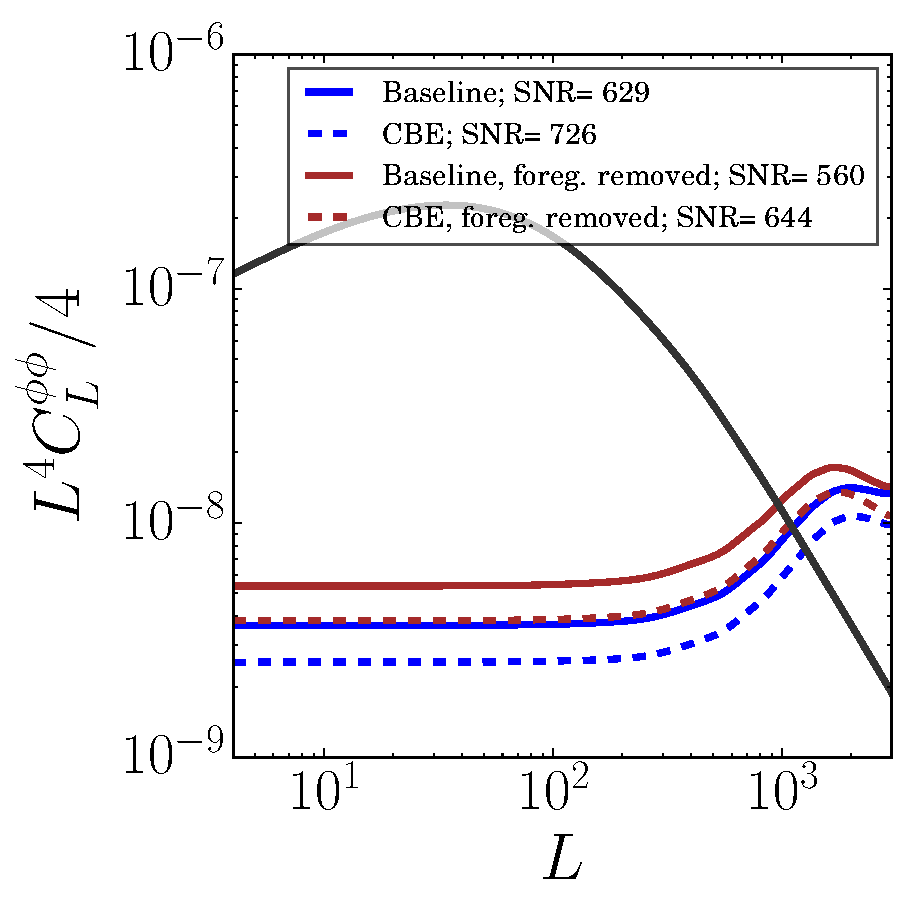
\includegraphics[width=3.0in]{images/lensingNoisePICO.pdf} } }
\hspace{0.in}
\parbox{3.5in}{
\caption{\label{fig:lensingNoisePICO} Lensing noise curves for various experimental configurations, showing the noise per mode of the reconstructed lensing field.  The signal curve, i.e., the CMB lensing power spectrum, is shown in grey; mapping of the matter density field is possible on scales where the noise curves fall below this signal.  Shown in solid are the performance of the $EB$ polarization estimator, including iterated delensing; this estimator performs best on large angular scales.  On smaller angular scales the temperature ($TT$) estimator shows the best performance. The associated signal to noise ratio for the lensing power spectrum is 570 for the 'requirement' configuration and 650 for the 'CBE' configuration. \textbf{Update with foreground-cleaned polarization noise curve(s) to demonstrate robustness.} } }
\vspace{-0.1in}
\end{figure}


%Measurements of the CMB reveal structure imprinted not only at the early time of recombination, but also at nearly every significant ensuing epoch in cosmic history.  In particular the matter between us and the CMB last-scattering surface will deflect the path of CMB photons, a process known as gravitational lensing.  Although the lensing of the CMB is a weak signal, targeted statistical estimators enable its extraction.  Measurements of the lensing signal have rapidly progressed, from the first detections in 2007-8 \citep{2007PhRvD..76d3510S, 2008PhRvD..78d3520H} to the recent $40\sigma$ measurement by the {\it Planck} team \cite{2018arXiv180706210P}.  When applied to a rich dataset such as that expected from the PICO satellite, these estimators will provide a map of all the matter in the Universe in projection, with the most sensitivity at redshift $z \simeq 2$ and down to scales of approximately ten arcminutes.  

%Forecasts show that the power spectrum of lensing in the PICO CMB map can be detected at approximately 580$\sigma$ or 650$\sigma$ for the requirement or CBE configurations, respectively.  Such high-S/N measurements are more than an order of magnitude improvement over the current state of the art, obtained by the {\it Planck} team.  The legacy value of the PICO CMB lensing map is immense, as has already been seen with {\it Planck}, particularly through the high-S/N cross-correlation science that will be enabled.  For example, tomographic cross-correlations of the PICO CMB lensing map with samples of galaxies and quasars will yield constraints on structure formation out to redshifts inaccessible to galaxy surveys or galaxy weak lensing maps on their own.  These measurements will yield constraints on dark energy, modified gravity, and neutrino mass (complementary to the neutrino mass inferred from the CMB lensing auto-power spectrum described earlier).  In addition, PICO CMB lensing cross-correlations will yield constraints on the properties of quasars and other high-redshift astrophysics, e.g., a precise determination of the quasar bias (and hence host halo mass) as a function of their properties, such as (non-)obscuration.  We provide further quantitative cross-correlation forecasts below.  Fig.~\ref{fig:lensingNoisePICO} shows per-mode noise curves for the reconstruction of CMB lensing from PICO, demonstrating the wide range of angular scales over which the matter density field will be mapped.  \textbf{Add brief discussion of foreground robustness demonstrated in Fig.~\ref{fig:lensingNoisePICO}}

{\bf Gravitational Lensing as Noise for Gravity Wave Science}

\comor{\SH version, need to reconcile with the paragraph below. } 
When the tensor to scalar ratio $r \simeq 0.01$, the B-mode lensing power spectrum and the one from gravity waves have approximately 
the same level at $\ell = 80$. For lower levels of $r$, the stronger gravity wave peak is masked by E-mode photons that are lensed into B. 
But the B-mode maps can be `delensed'~\cite{??}. The effect of lensing on E and B maps can be determined and undone if these maps are 
measured with few arcmin resolution and with sufficient depth. Forecasts show that at a minimum 73\% of lens-induced $B$ mode power will 
be removed for the PICO 'requirement' configuration, after accounting for foreground subtraction. 80\% will be removed if the foregrounds 
do not degrade the inherent SNR, rising to 85\% for the CBE. Without delensing PICO determination of $r$ would be limited to $r>??$. 
We emphasize that PICO will be relying on its own data to conduct the delensing and foreground cleaning, thus avoiding reduced efficacy arising 
from the need to cross-calibrate experiments, identify common observing areas on the sky, or not having frequency band coverage at the appropriate resolution to remove foregrounds. 


\comor{AVE version}
Lensing breaks the highly symmetric configuration of primordial density fluctuations appearing as $E$ modes on the sky, turning some of these into $B$ modes.  If not accounted for, this effect yields a noise floor on the large-scale $B$ modes that can be measured from the early Universe.  However, maps of $E$ modes and of the lensing field, both of which will be obtained with PICO data, can be used together to create a template for these lensed $B$ modes.  This template can then be subtracted from the measured $B$ modes to obtain improved performance, in a process known as ``delensing'' \citep{2004PhRvD..69d3005S,2012JCAP...06..014S}.  Forecasts show that up to 80\% of the lens-induced $B$ mode power can be removed in the 'requirement' configuration, with this number becoming 85\% for the current best estimate.  

\textbf{To be added:}

\textbf{- CMB halo lensing forecast (Jim, Jean-Baptiste)}

\textbf{- Cross-correlation forecast (Marcel)}


{\bf Physics of Galaxy Formation via the Sunyaev-Zel'dovich (SZ) Effects}

Not all CMB photons propagate through the universe freely; about 6\% are Thomson-scattered by free electrons in the intergalactic medium (IGM) and intracluster medium (ICM). These scattering events leave a measurable imprint on CMB temperature fluctuations, and they contain a wealth of information from how structure grows to the thermodynamic history of baryons. A fraction of these photons are responsible for the Sunyaev--Zel'dovich effects~\citep{SZ1969,SZ1972}. The thermal SZ effect (tSZ) is the increase in energy of CMB photons due to scattering off hot electrons. This results in a spectral distortion
%, proportinal to the electron pressure,
 of the CMB blackbody that corresponds to a decrement in CMB temperature at frequencies below 217 GHz and an increment at frequencies above. The kSZ effect is the Doppler shift of CMB photons Thomson-scattering off free electrons that have a non-zero peculiar velocity with respect to the CMB rest frame. 
%This produces small shifts in the CMB temperature proportional to the radial velocity of the object and its optical depth.
The amplitudes of the tSZ and kSZ signals are proportional to the integrated electron pressure (tSZ) and momentum (kSZ) along the line of sight, respectively.  They thus contain information about the thermodynamic properties of the IGM and ICM.
%since their magnitudes are proportional to the integrated electron pressure (tSZ) and momentum (kSZ) along the line of sight.
The tSZ effect can be used to measure ensemble statistics of galaxy clusters, which contain cosmological information, as well as to provide uniform cluster samples for galaxy formation studies in dense enviroments.
%
%\item Cosmological parameters from the abundance of tSZ-detected clusters and statistics of component-separated tSZ maps.
%\item Thermodynamic properties of galaxies, groups, and clusters from combined tSZ and kSZ cross-correlation measurements.
%\item Measurements of peculiar velocities, which are powerful cosmological probes on large scales, through the kSZ effect.
%\item Patchy reionization which imprints the CMB through higher order moments of the kSZ effect.

{\bf Galaxy Clusters}

%Through the tSZ PICO will produce a large all sky catalog of 

Galaxy clusters found via the tSZ  effect provide a well-defined sample with a simple-to-model selection function. Sample of clusters such as these are easy to use for cosmological inferences and studies of galaxy evolution in dense environments. 
Points to still hit.
High z sample,
Numbers -- Nick and Jim should cross-check,
most massive cluster all over the whole sky,
Cosmology.

{\bf Compton-$y$ map and tSZ auto-power spectrum}

In addition to finding individual clusters, multifrequency CMB data also allow the reconstruction of full-sky maps of the thermal SZ signal (Compton-$y$ maps) via foreground removal algorithms similar to those used to obtain cleaned maps of the CMB.  With its extremely low noise and broad frequency coverage, PICO will yield a definitive Compton-$y$ map over the full sky, with high S/N down to angular scales of a few arcminutes.  We quantify this expectation by reconstructing the Compton-$y$ field using the needlet internal linear combination (NILC) algorithm~\cite{Delabrouille2009} applied to sky simulations generated with the \planck sky model, with maps at all PICO frequencies (with appropriate noise added).  The error bars on the reconstructed tSZ power spectrum are shown in Fig.~\ref{fig:PICO_tSZ_PS}, in comparison to current measurements.  The total $S/N = 1270$ for the PICO CBE configuration, with the PICO requirements configuration only $\approx 10$\% lower.  This is nearly two orders of magntiude larger than the current S/N from \planck.

Extremely strong constraints on models of astrophysical feedback will be obtained from the analysis of the PICO $y$-map, both from its auto-poewr spectrum and from cross-correlations with galaxy, group, cluster, and quasar samples.  Like the CMB lensing map described above, the legacy value of the PICO $y$-map will be immense.  As an example, we forecast the detection of cross-correlations between the PICO $y$-map and galaxy weak lensing maps constructed from LSST and WFIRST data.  Considering the LSST ``gold'' sample with a source density of 26 galaxies/arcmin${}^2$ covering 40\% of the sky, we forecast a detection of the tSZ -- weak lensing cross-correlation with S/N = 3000.  At this immense significance, the signal can be broken down into dozens of tomographic redshift bins, yielding a precise breakdown of the evolution of thermal pressure over cosmic time.  For PICO and WFIRST (assuming 45 galaxies/arcmin${}^2$ covering 5.3\% of the sky), we forecast S/N = 1100 for the tSZ -- weak lensing cross-correlation.  The WFIRST galaxy sample extends to higher redshift, and thus this high-S/N measurement will allow the evolution of the thermal gas pressure to be probed to $z \approx 2$ and beyond, the peak of the cosmic star formation history.  These transformative measurements will revolutionize our understanding of galaxy formation and evolution by distinguishing between models of feedback energy injection at high significance.  Additional cross-correlations of the PICO $y$-map with quasar samples, filament catalogs, and other large-scale structure tracers will further demonstrate its immense legacy value.

\begin{figure}
\begin{center}
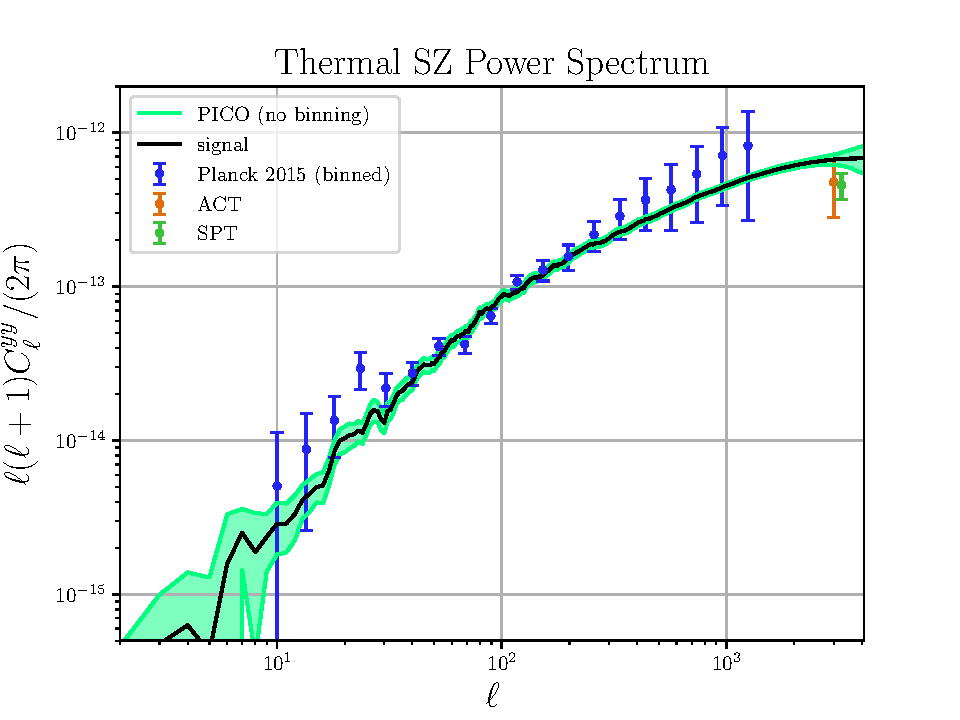
\includegraphics[width=0.8\textwidth]{images/PICO_tSZ_PS_plot.pdf}
\end{center}
\caption{\label{fig:PICO_tSZ_PS} Constraints on the tSZ power spectrum from PICO and current data.  The black curve shows the simulated tSZ power spectrum signal.  The light green shaded region shows the error bars for PICO at each multipole, i.e., with no binning, as determined from NILC analysis of full-sky simulations.  The blue points show the current constraints from Planck, which have been averaged into broad multipole bins.  The orange and dark green points show the constraints from ACT and SPT, respectively, at a single multipole of $\ell=3000$.  The overall PICO $S/N = 1270$, nearly two orders of magnitude larger than current measurements.}
\end{figure}


\end{document}

%\begin{figure}[!htb]
%\centering
%
\includegraphics[width=4cm]{images/example}
%\caption{example}
%\label{fig:im_3}
%\end{figure}
